\documentclass[_main.tex]{subfiles}
 
\begin{document}

\section*{A framework for analysing the coalescent process}  
\label{main_coalescent}

The idealised genomic transmission graph naturally lends itself to coalescent analysis.  To start with a simple example, consider the special case of a parasite population with no superinfection, i.e. $\chi =0$.  We shall sample two alleles at a point locus and follow their lineages back in time until they coalesce in a common ancestral allele, as illustrated in figure \ref{fig:coalescent}.  Let \textbf{T} be a random variable representing time to coalescence of the two alleles.

\begin{figure}[h!]
\centering
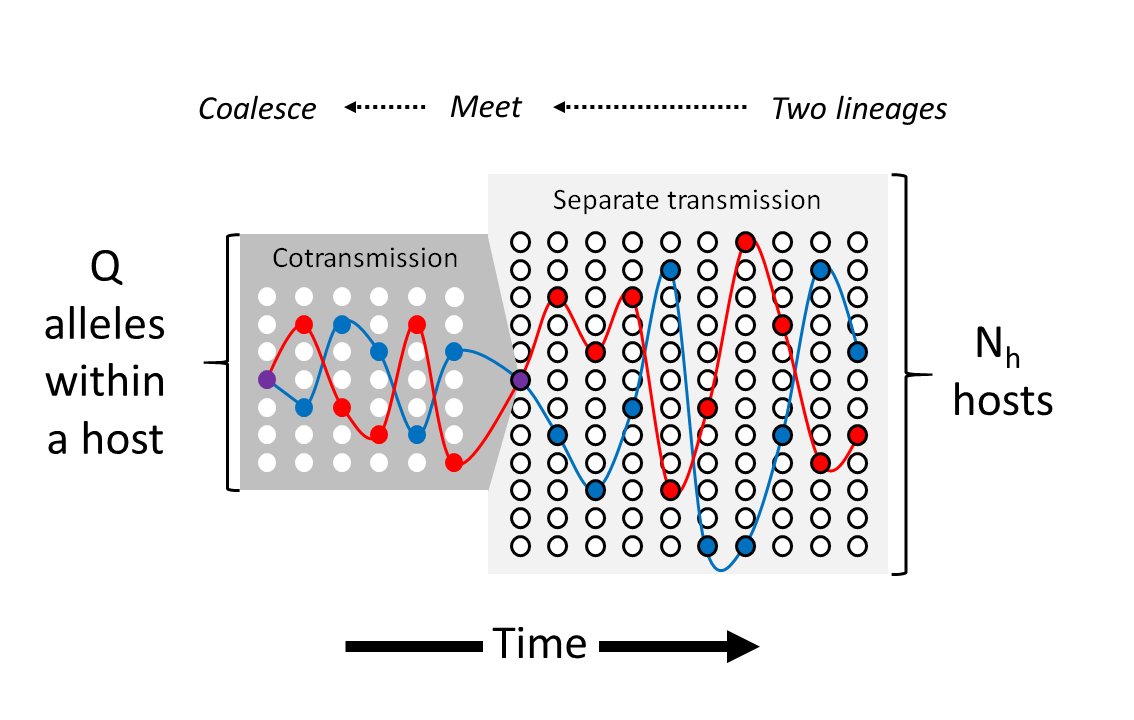
\includegraphics[width=12cm]{180929a_tg_coalescence.png}
\caption{\textbf{Coalescence of two lineages in the absence of superinfection}. Each column represents one generation of the transmission graph: the light grey block on the right represents all hosts and the dark grey block on the left represents the within-host population of a single host.    Imagine that we sample two alleles from different hosts (red and blue circles on the far right) and follow their lineages back in time.  The two lineages remain in separate transmission chains for several generations until they meet in a common host.  They are then cotransmitted until they coalesce in a common ancestral allele (purple circle on the far left).}
\label{fig:coalescent}
\end{figure}

If we sample two alleles from different hosts in the same generation, they are by definition on \textit{separate transmission chains}, but if we trace their lineages back in time they will eventually \textit{meet} in a common host.  Once that has happened, the two lineages are \textit{cotransmitted} along the same transmission chain until they eventually \textit{coalesce} in a common ancestral allele. 

If two lineages are on separate transmission chains at a particular point in time, there is a probability of $1/N_h$ that they meet in a common host when we go back one generation.  If two lineages are cotransmitted, there is a probability of $1/Q$ that they coalesce when we go back one generation.  As described in Methods section \ref{supp_coal_chi_zero} from this we can obtain the expectation of time to coalescence:

\begin{equation*}
\label{eq:Nh+Q-1}
E \{ \textbf{T} \}   
= N_h + Q - 1
\end{equation*}

Thus if $\chi=0$ and $Q = 1$ then two alleles have an expected coalescence time of $N_h$ generations, equivalent to a Wright-Fisher population of $N_h$ haploid parasites.  Likewise, if $\chi=0$ and $N_h = 1$ then two alleles have an expected coalescence time of $Q$ generations, equivalent to a Wright-Fisher population of $Q$ haploid parasites.  Thus we can view the standard Wright-Fisher model as a special case of the genomic transmission graph.

%%%%%%%%%%
\paragraph{Mapping the coalescent onto the transmission graph.}
\label{main_map_coalescent}
%%%%%%%%%%

We shall now consider the general case of a parasite population in which superinfection can occur, i.e. $\chi \ge 0$.  As in the previous section, we sample two alleles at a point locus and follow their lineages back in time, but the journey to coalescence is more complicated.  As illustrated in figure \ref{fig:graph_1}, this can be broken down into three stages:

\begin{figure}[h!]
\centering
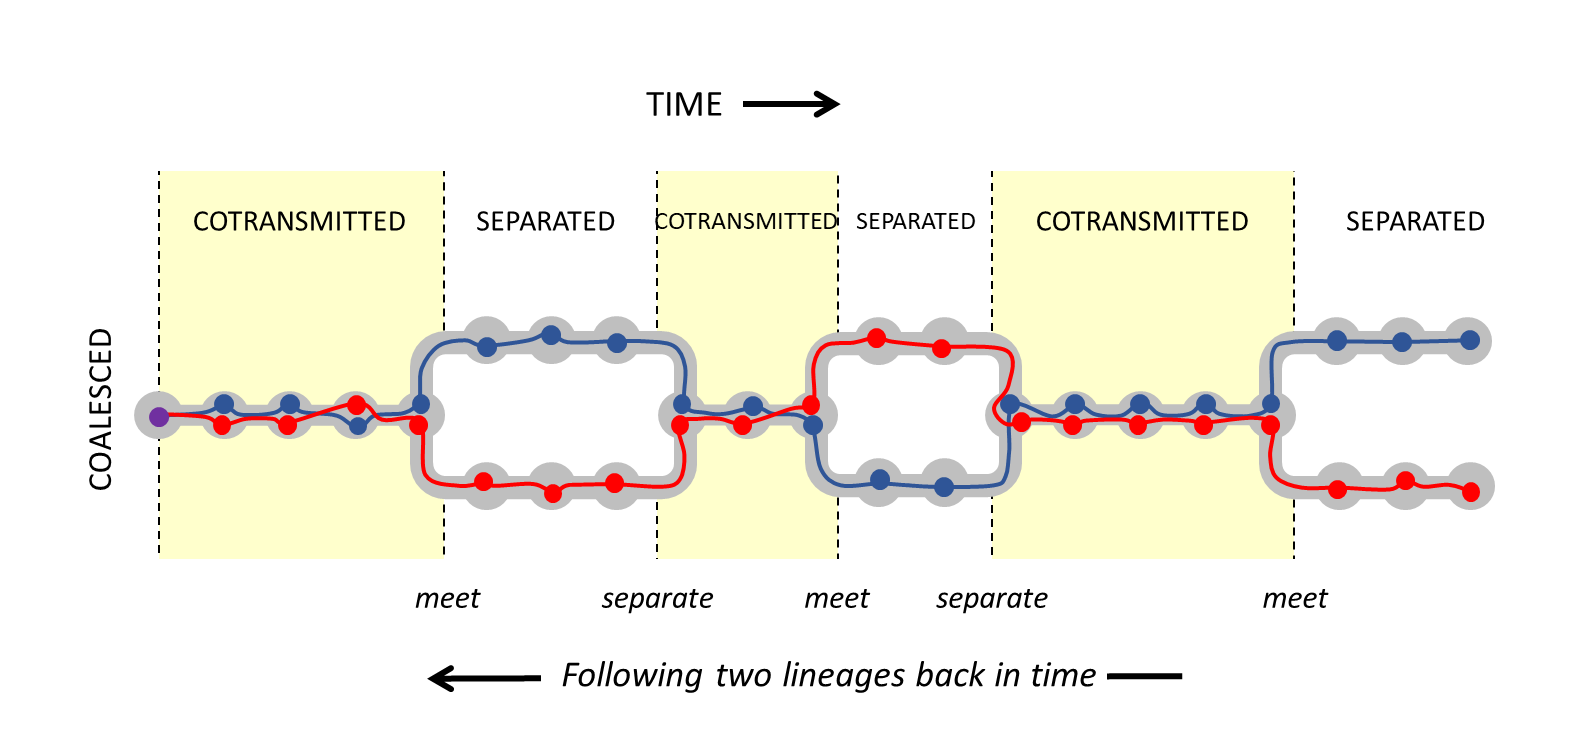
\includegraphics[width=15cm]{181003_tg_lineage.png}
\caption{\textbf{A graph of coalescing lineages}.  Imagine that we sample two alleles from different hosts, as depicted by the red and blue circles on the far right.  The corresponding lineages (red and blue lines) can be mapped onto specific transmission chains (thick grey lines) and individual hosts (grey blobs).   Proceeding back in time, the corresponding lineages occasionally meet in the same host and are cotransmitted for a period of time before separating again to different hosts.  Eventually they meet and coalesce in a common ancestral allele represented by the purple circle on the far left.}
\label{fig:graph_1}
\end{figure}

\begin{enumerate}

\item When we sample two alleles from different hosts in the same generation, at that point in time they are on separate transmission chains, but if we trace their lineages back in time they will eventually meet in the same host. 

\item Once the lineages have met in the same host, as we proceed further back in time they are \textit{cotransmitted} along the same transmission chain until one of two events occurs:

\begin{enumerate}

\item The two lineages \textit{coalesce} in a common ancestral allele.

\item The two lineages \textit{separate} onto different transmission chains.

\end{enumerate}

\item If the two lineages separate at stage 2, then we are effectively back at stage 1 and we must wait again for the two lineages to meet in the same transmission chain before they have the possibility of coalescing.

\end{enumerate}

It will be evident that we are dealing with an iterative loop that might need to be repeated for multiple cycles before the two lineages eventually coalesce.  If we consider all the possible ways in which two lineages could progress through the transmission graph, at any point in time the system must be in one of three states:

\begin{itemize} [noitemsep]

\item \textsc{separated} - the two lineages are in different hosts

\item \textsc{cotransmitted} - the two lineages are in the same host

\item \textsc{coalesced}

\end{itemize}

We can write down the probability of transition between these three states if we follow two lineages back in time by one generation.  For example, if two lineages are separated and we go back one generation, there is a probability of $1/N_h$ that they will meet in the same host and, if they do so, then there is a probability of $1/Q$ that they will coalesce in that host.

\begin{equation*} \label{eq:coal3}
\Pr \{ \textsc{\small{separated}} \rightarrow \textsc{\small{coalesced}} \} 
= \frac{1}{N_hQ}
\end{equation*}

To give another example, if two lineages are cotransmitted and we go back one generation, they will separate onto different transmission chains if their current host is superinfected ($\Pr = \chi$) and they come from different source hosts ($\Pr = Q/(2Q-1)$).

\begin{equation*} \label{eq:coal4}
\Pr \{ \textsc{\small{cotransmitted}} \rightarrow \textsc{\small{separated}} \} 
= \frac{Q\chi}{2Q-1}
\end{equation*}

In a similar manner we can define the transition probabilities for all possible states of two lineages when we go back in time by one generation, as described in Methods section \ref{supp_coalescent}, and the results are given in Table \ref{tab:main_tr_matrix}.

\renewcommand\theadalign{bc} 

\begin{table}[h!] 
\centering
\large{
\begin{tabular}{l | c c c } 
\hline \\
\textbf{\small{State}} & \small{Separated} & \small{Cotransmitted} & \small{Coalesced} \\ [0.5ex] 
\hline \\
\small{Separated} & $1 - \frac{1}{N_h}$ & $\frac{1}{N_h} (1 - \frac{1}{Q})$ 
& $\frac{1}{N_hQ}$ \\ [2ex]
\small{Cotransmitted} & $\frac{Q\chi}{2Q-1}$ & $\frac{(Q-1)(2Q - Q\chi - 1)}{Q(2Q-1)}$
& $\frac{2Q - Q\chi - 1}{Q(2Q-1)}$ \\ [2ex] 
\small{Coalesced} & 0 & 0 & 1 \\ [1ex]  
\hline
\end{tabular}
}
\caption{\small{\textbf{Transition probabilities for the three possible states of two lineages}. At any point in time, two lineages must be (1) separated or (2) cotransmitted or (3) coalesced. Row $i$ column $j$ of the table gives the probability that lineages in state $i$ will transition to state $j$ if we go back a single generation.  By definition, the probabilities in each row sum to 1.}}
\label{tab:main_tr_matrix}
\end{table}

%%%%%%%%%%%%%%%%%%%%%%%%%%%%%%%%%%%%%%%%

\paragraph{Markov chain simulation of time to coalescence.}  \label{main_mcs}

Table \ref{tab:main_tr_matrix} gives us a transition probability matrix that allows us to evaluate the state of two lineages at any point in time by Markov chain simulation (Methods section \ref{supp_mcs}).  We start the simulation by sampling two imaginary alleles at a point locus, and then following their lineages back in time through the generations.  To study between-host variation we imagine that the two alleles are sampled from different hosts, i.e. the two lineages are separated at the start of the simulation. Alternatively, we can study within-host variation by imagining that the two alleles are sampled from the same host, i.e. the lineages are cotransmitted at the start of the simulation.  From this we can calculate the probability distribution of coalescence time for two alleles, sampled either between-host or within-host, as illustrated in figure \ref{fig:main_markov_4}.   

\begin{figure}[h!]
\centering
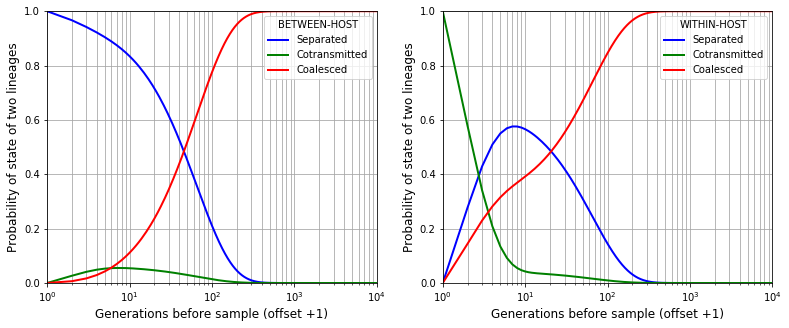
\includegraphics[width=15cm]{221029_tc_dist.png}
\caption{\textbf{State of two lineages as we proceed back in time after sampling two alleles.}  If we sample the alleles from different hosts (\textbf{left panel}) then the lineages are initially separated (blue) but over time there is an increasing probability that they are cotransmitted (green) and eventually they coalesce (red).  If we sample alleles from the same host (\textbf{right panel}) then the lineages are initially cotransmitted. In this example the transmission parameters are $N_h=30$, $Q=5$, $\chi=0.5$.  The horizontal axis is offset by +1 to allow the use of a log scale. \href{https://d-kwiat.github.io/gtg/coalescence-time-basic.html}{See worked example}.
}
\label{fig:main_markov_4}
\end{figure}

The probability distribution of coalescence times depends on the combination of transmission parameters, and it contrasts with the classic Wright-Fisher coalescent process which invariably gives a geometric distribution.  In the case of between-host variation (figure \ref{fig:main_markov_3} upper panels), when $Q>1$ the rate of coalescence tends to increase over the first few generations, and depending on $\chi$ it may then stay fairly constant for some time before declining asymptotically to zero.

\begin{figure}[h!]
\centering
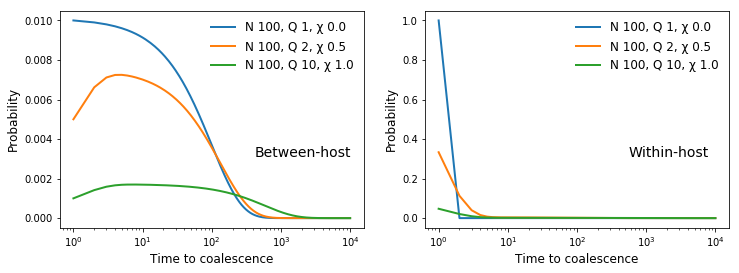
\includegraphics[width=15cm]{221029_tc_examples.png}
\caption{\textbf{Between-host and within-host times to coalescence.}  We use a Markov process to compute the probability distribution of coalescence times for two alleles sampled from different hosts (\textbf{left panel}) or from the same host (\textbf{right panel}) for different combinations of transmission parameters.  Note that the two panels have markedly \textbf{different scales}, and that two alleles sampled from the same host coalesce much more rapidly than two alleles sampled from different hosts when $\chi=0$, whereas the difference is less marked when $\chi=1$.
}
\label{fig:main_markov_3}
\end{figure}

In general, two alleles sampled from the same host coalesce more rapidly than two alleles sampled from different hosts.  The difference is marked when $\chi=0$.   As $\chi$ increases, the coalescence time of two alleles sampled from the same host starts to approach that of two alleles sampled from different hosts, and when $\chi=1$ the difference becomes relatively small.  An exception to this general rule is discussed in Methods section \ref{supp_anomaly}.

\end{document}